% Chapter Template

\chapter{Introduction} % Main chapter title

\label{Chapter1} % Change X to a consecutive number; for referencing this chapter elsewhere, use \ref{ChapterX}

%----------------------------------------------------------------------------------------
%	SECTION 1
%----------------------------------------------------------------------------------------
Imaging is a process that we are doing all time, we have a pair of optical systems (OS) that are mapping
constantly, and doing a recreation of the things around us. This pair of OS is what we call eyes, 
without them we would be able just to \textit{fell} what surround us, it would be impossible to \textit{see}, to do an
\textit{image} of our surroundings. The components of the eye are a well stablished optical system, this OP 
uses the light that is reflected or scattered from the objects and then comes towards the eye. At the
back of the eye we have a photodetector that is called Retina, it converts the photons into electrical
signals that travels through our Brain, where the image is then recovered. Figure \ref{fig:eye} show a really 
simplified schematics of the eye seen as an OS.

\begin{figure}[h!]
\centering
\label{fig:eye}
 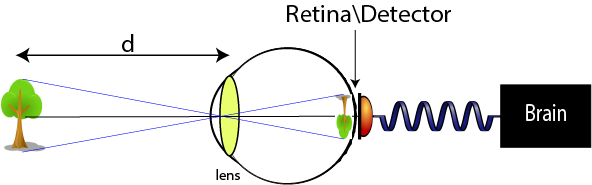
\includegraphics[width=0.65\textwidth]{Figures/eye.png}
 \caption{Eye seen as a Optical System} 
\end{figure}


For taking a photograph of an object, traditionally, we need to face a camara detector (CCD) to the object, 
in a similar way we have to point our eyes to the objects we are seeing, Figure \ref{fig:eye}.
Both retina and CCD saves some kind of the spatial shape of the light that comes through.
This spatial information is necessary then for the process of reconstructing an image of an object, from this
statment we can start talking about a spot-to-spot correspondence between the object and the image plane.
It is important to point out that we usually make images, 2D representations, of 3D objects. For this
reason we talk about an image plane, which is the plane where, depending on the OS, the 2D representation
of the object is going to be formed. 


What would happen if our retina or CCD stoped saving this spatial references?, if our retina now is 
only able to detect that light is going through, not where. It is clear that in this situation 
the imaging process would be imposible, without any spatial information is not posible to create a representation in 2D of something.

Two-photon imaging is techniche that could solve this dilema. It is also a optical imaging experiment 
that started to draw attention after Pittman's first realisation \cite{pittman}. As the name suggest it, 
Two-photon imaging, we use a second photon to reconstruct the image. In other words, in order to reconstruct
an image we use two detectors that are spatially separated. In this opportunity we use a detector that
is toward the light source $D_A$ and another detector $D_B$ that is towards the object. In Figure
\ref{fig:twoPh} there is schematic of the situation, we collect the light from the source and after 
the object, in this case a double slit. Where $D_B$ is a big detector that collects all the light after the object, 
while $D_A$ is a small detector that is capable of scanning the transverse direction of the light propagation. 
\begin{figure}[h]
\centering
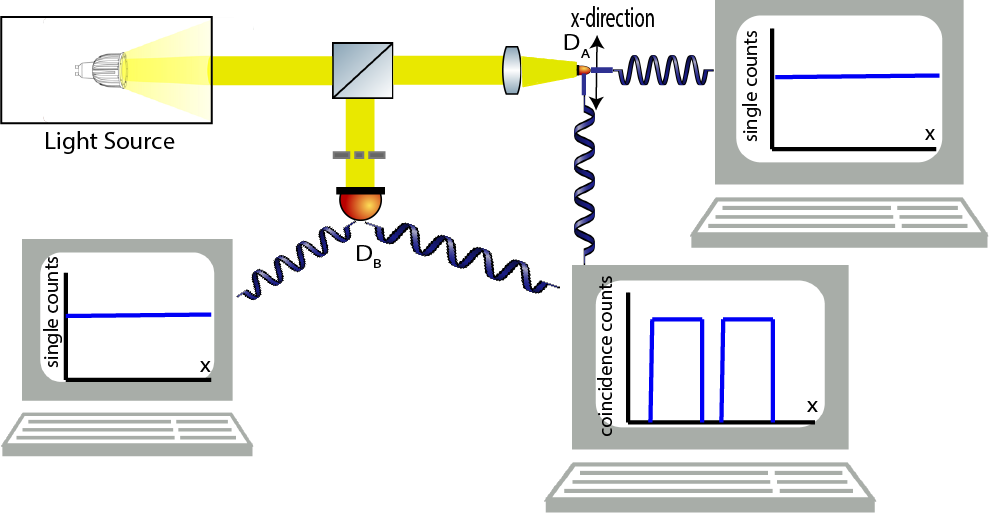
\includegraphics[width=0.75\textwidth]{Figures/twoPhotonSetup.png}
\caption{Two-photon imaging techniche setup} 
\label{fig:twoPh}
\end{figure}

There are different types of Two-photon imaging, and they differs from each other in the nature of the light 
source used. The first two-photon imaging realisation used entangled photon pairs as the light source. In 1995 Pittman, realized a 
quantum two-photon geometric optical effect.  They have successfully performed optical 
imaging by means of a quantum-mechanical entangled source\cite{pittman}.

The second kind of imaging uses chaotic light. This light can be understood as the radiation coming from
a blackbody at thermal equilibrium in temperature, it means the light source is composed by 
a huge number of photons and they are randomly distributed in the posible momentum and frequencies.
this is because each photon corresponds to a transition in one of the trilion atoms or molecules of the light source.
Valencia \textit{et al.} where the first ones to present a experimental demonstration 
of two-photon ghost imaging with thermal-like sources\cite{thermalAlejandra}.

It is possible to reconstruct the image in this two experiments because there is some king of 
correlation between the photon that are generated from the source, in the quantum light source, there
is entanglement between the pair of used photons. Depending in certains situations we can say the 
pair is anti-correlated\cite{broke}. In the experiment of the chaotic light, the source is 
modeled as an incoherent statistical mixture of many pairs of photons; the various two-photon 
probability amplitudes are provided by the entire ensemble of photon pairs. There is a correlation
between this probability amplitudes that allows to retrive the image.

In our experiment we have done a Two-photon imaging using a source of entangled photons, we are able
to change the how the generated photons are entangled, more specifically, we can tune 
the way the transverse momentums $\vec{q}_A$ and $\vec{q}_B$ are correlated. Changing the shape of this
spatial correlation will have an effect in the obtained image. The pair of photons are created by 
focusing a laser beam to a nonlinear crystal, this process is named SPDC. We control the shape
of the spatial correlations by changing the pump waist of the laser. This monograph intend to describe
this experiment and develop the theory behind it, also show some hits about the possible 
effects of the different spatial correlations in the image.

As pointed out before, this experiment consist in a source light and two arms, one that interacts 
with an object, path $B$, and another that propagates through free space, path $A$.So this last one 
can be simulated by a computer using Fresnel's propagation theory, doing so is called the Computational 
Two-photon Imaging. It allows us to simulate the electric field data, to be obtain it before, during 
or after the data from the reflected arm is generated ($B$),eliminating the need for collecting 
the data generated in the transmitted path ($A$). Also we have to use less opto-electronical 
elements on the optical table, simplifying the original setup and reducing considerably 
the amount of data generated. The resulting detection module consist only in one detector, a bucket detector that collects
 a single pixel (no spatial information) on light which has been transmitted through or reflected from the object.
In this situation only one light beam and one photodetector are required, this means that this imaging configuration cannot depend
on non-local two-photon interference\cite{simulated}.



This document is organized as follows: Chapter 2 presents a theoretical discution about the fundamental 
aspects of the two-photon imaging, with an especial focus on the SPDC generation of entangled photons, and
the imaging using this pairs as the source light. 
In chapter 3 there is a meticulous explanation of the experimental setups used in this monograph,
explaining each element used in the optical table.The experimental results are presented in the 
chapter 4. The conclusions and further discussion are on chapter 5.

